\documentclass[sigplan,screen]{acmart}

\usepackage{booktabs} % For formal tables
\usepackage{bm}
\usepackage{hyperref}
\usepackage{fontspec}
\usepackage[utf8]{inputenc}

% TOG prefers author-name bib system with square brackets
% \citestyle{acmauthoryear}
%\setcitestyle{nosort,square} % nosort to allow for manual chronological ordering
\settopmatter{printacmref=false}
\acmBooktitle{CSC417 Physics-Based Animation}
\acmConference{CSC417 Physics-Based Animation}{2020}{Toronto, ON, Canada}

\begin{document}

\title[2D Fluid/Smoke Simulation in WebGL using GLSL]{Two-Dimensional Fluid/Smoke Simulation in WebGL using the OpenGL Shading Language}

\author{David Vajcenfeld}
\affiliation{%
 \institution{University of Toronto}
 \streetaddress{27 King's College Circle}
 \city{Toronto}
 \state{ON}
 \postcode{M5S 1A1}
 \country{Canada}}
\email{david.vajcenfeld@mail.utoronto.ca}

\renewcommand\shortauthors{Vajcenfeld D.}

\begin{abstract}
This paper describes an implementation of fluid and smoke simulation in WebGL,
a web-based graphics library based on OpenGL.
The Navier-Stokes equations are used to govern fluid, 
and calculated using separate shader programs on the GPU.
The Poisson pressure equation is estimated using the iterative Jacobi method. 
\end{abstract}

%
% Generated by http://dl.acm.org/ccs.cfm.
%
\begin{CCSXML}
    <ccs2012>
    <concept>
    <concept_id>10010147.10010371.10010352.10010379</concept_id>
    <concept_desc>Computing methodologies~Physical simulation</concept_desc>
    <concept_significance>500</concept_significance>
    </concept>
    </ccs2012>
\end{CCSXML}
\ccsdesc[500]{Computing methodologies~Physical simulation}

\keywords{Fluid simulation, smoke simulation, WebGL, GLSL, shaders.}

\maketitle

\newcommand{\dt}{\Delta t}

\section{Introduction}

This paper describes an implementation of fluid and smoke simulation in WebGL.
The Web Graphics Library, commonly referred to as WebGL, is a JavaScript API
for ``high-performance interactive 2D and 3D graphics'' \cite{webgl} that can easily be viewed 
in modern web browsers. 
It is based on OpenGL ES 2.0 and makes use of the OpenGL ES Shading Language (GLSL ES).

In this project, a fluid and smoke simulation in two dimensions was implemented,
by solving the Navier-Stokes equations.

\section{Related Work}

The \textit{Fluid Simulation} course notes from SIGGRAPH 2007 go into detail on the
Navier-Stokes equations, 
how they are split into components for computation,
and how the pressure equation is solved in both two and three dimensions. \cite{fluid}

The \textit{GPU Gems} book, and more specifically chapter 38 \textit{Fast Fluid Dynamics Simulation on the GPU},
goes into the details on fluid simulation in two dimensions using shaders.
This project primarily attempts to implement this in WebGL. \cite{nvidia}

The paper \textit{Smoke Simulation using WebGL Technology} covers generally the same content
as the chapter in the \textit{GPU Gems}, but implemented in WebGL and in three dimensions.
Most importantly, it provides details on how the approach is extended to three dimensions.
\cite{smokesim}

Finally, the \textit{WebGL Fluid Simulation} code repository by Pavel Dobryakov implements a similar 
smoke-like fluid simulation in WebGL.
This code repository was used initially as a reference as a basis on how WebGL was set up 
and interacted with the shaders, as the author if this project was greatly unfamiliar with the works of WebGL.
Similarly, the idea and implementation of ``splattering'' fluid particles by mouse click-and-drag
was taken from here.
\cite{webglsim}

\section{Method}

The Navier-Stokes equations consist of a set of partial differential equations (PDEs) that 
govern the motion of simulated viscous fluids and smoke. \cite{fluid}

In WebGL, we implement this as a set of WebGL programs written in GLSL and executed on the GPU. 
Each program consists shaders which
operate on the level of a single pixel or texel, respectively.
A texel is a texture pixel, the smallest component of a texture map,
which we use to represent fluid particles in our simulation.
This paper will refer to ``texel'' and ``pixel'' interchangeably.

We solve the Navier-Stokes equations analytically by splitting them into a series 
of computational steps by the Helmholtz-Hodge Decomposition. 
These are then implemented as individual shader programs,
and their values computed onto a set of framebuffers which represent various quantities.
Framebuffers are matrices that contain a four-vector for each texel in our simulation. 

\subsection{Advection Program}

This program handles the advecting (i.e.\ transporting) of the fluid particles
by applying their velocities.

Traditionally this would be done by computing the position of a particle after 
the time step as in \autoref{eqn:adv-std}, and moving it appropriately.
\begin{equation}\label{eqn:adv-std}
  \bm{x}(t+\Delta t)=\bm{x}(t) + \dt \bm{v}(t)
\end{equation}
Instead, in the fragment shader of the advection program we trace the position of each texel to its 
position in the previous time step, and then copy the values over from there, as in \autoref{eqn:adv}.
In \autoref{eqn:adv}, $c(\bm{x})$ represents either the velocity or the density at position $\bm{x}$,
as this advection program is executed on both the velocity and density framebuffers.
\begin{equation}\label{eqn:adv}
  c(\bm{x}) = c(\bm{x} - \dt \bm{v}(t))
\end{equation}

\subsection{Divergence Program}

This program calculates the divergence of the vector field $\nabla \cdot \bm{v}$
as the first step in solving the pressure equation,
by using the discrete equation in \autoref{eqn:div}.
\begin{equation}\label{eqn:div}
  \nabla \cdot \bm{v} = \frac{v_{i+1,j}-v_{i-1,j}}{2\Delta x}+\frac{v_{i,j+1}-v_{i,j-1}}{2\Delta y}
\end{equation}
In \autoref{eqn:div}, $\Delta x$ and $\Delta y$ represent the ``space step'' in the two dimensions.
In our case this is the same in both dimensions, so we have $\Delta x = \Delta y$.

\subsection{External Forces Program}

This program just applies the effects of external forces that act on the liquid,
such as gravity or user input, onto the velocities of the particles,
using \label{eqn:f}, where $\bm{g}$ is the forces acceleration vector.
\begin{equation}\label{eqn:f}
  \bm{v}(t+\dt) = \bm{v}(t) + \dt \bm{g}
\end{equation}

\subsection{Jacobi Method Program}

This program is a simple iterative solver for the pressure equations.
This method, the Jacobi method, converges slowly, but is fast to execute on the GPU.
Consequently, we use around forty iterations to arrive at a sufficiently-accurate estimate.

The update-step equation used is \autoref{eqn:jacobi}, 
where $x$ is the pressure $p$, $b$ is the divergence $\nabla\cdot\bm{v}$,
and the parameters $\alpha=-(\Delta x)^2$ and $\beta=4$.
Also, $k$ represents the iteration.
\begin{equation}\label{eqn:jacobi}
  x_{i,j}^{(k+1)} = \frac{1}{\beta} \left( x_{i-1,j}^{(k)} + x_{i+1,j}^{(k)} + x_{i,j-1}^{(k)} + x_{i,j+1}^{(k)} + \alpha b_{i,j} \right)
\end{equation}

\subsection{Gradient Subtraction Program}

This program corrects the divergence of the velocity by subtracting the gradient of the pressure,
creating the divergence-free vector field $\bm{u}$, as seen in \autoref{eqn:grad-sub}.
\begin{equation}\label{eqn:grad-sub}
  \bm{u} = \bm{v} - \nabla \bm{p}
\end{equation} 

\subsection{Boundary Condition Program}

Finally, an important part of fluid simulation is to enforce conditions on the boundaries.
Here we update the velocities and pressures to satisfy the Neumann boundary conditions,
enforcing that the rate-of-change normal to the boundary is zero.

\autoref{eqn:bound-u} and \autoref{eqn:bound-p} show the velocity and pressure updates,
respectively, for particles on the left boundary.
The updates apply similarly to other the other boundaries.
\begin{equation}\label{eqn:bound-u}
  \frac{\bm{u}_{0,j}+\bm{u}_{1,j}}{2}=0 \implies \bm{u}_{0,j} = -\bm{u}_{1,j}
\end{equation}
\begin{equation}\label{eqn:bound-p}
  \frac{\bm{p}_{1,j}-\bm{p}_{0,j}}{\Delta x}=0 \implies \bm{p}_{0,j} = \bm{p}_{1,j}
\end{equation}

Below, in \autoref{eqn:bound-up}, we see the update logic performed by this program.
For velocity updates, $x$ represents the velocity and the scale is $s=-1$.
Similarly, for pressure updates $x$ represents the pressure and the scale is $s=1$. 
\begin{equation}\label{eqn:bound-up}
  x_{i,j} \gets \begin{cases}
      s \cdot x_{1,j} & \text{if}\ i=0\ \text{(left boundary)} \\
      s \cdot x_{W-2,j} & \text{if}\ i=W-1\ \text{(right boundary)} \\
      s \cdot x_{i,1} & \text{if}\ j=0\ \text{(top boundary)} \\
      s \cdot x_{i,H-2} & \text{if}\ j=H-1\ \text{(bottom boundary)} \\
      x_{i,j} & \text{otherwise}
  \end{cases}
\end{equation}

\section{Results}

As a result, we see a colorful simulation of a continuous fluid swirling around in
the WebGL canvas, as seen in \autoref{fig:result}.

\begin{figure}[H]
  \centering
  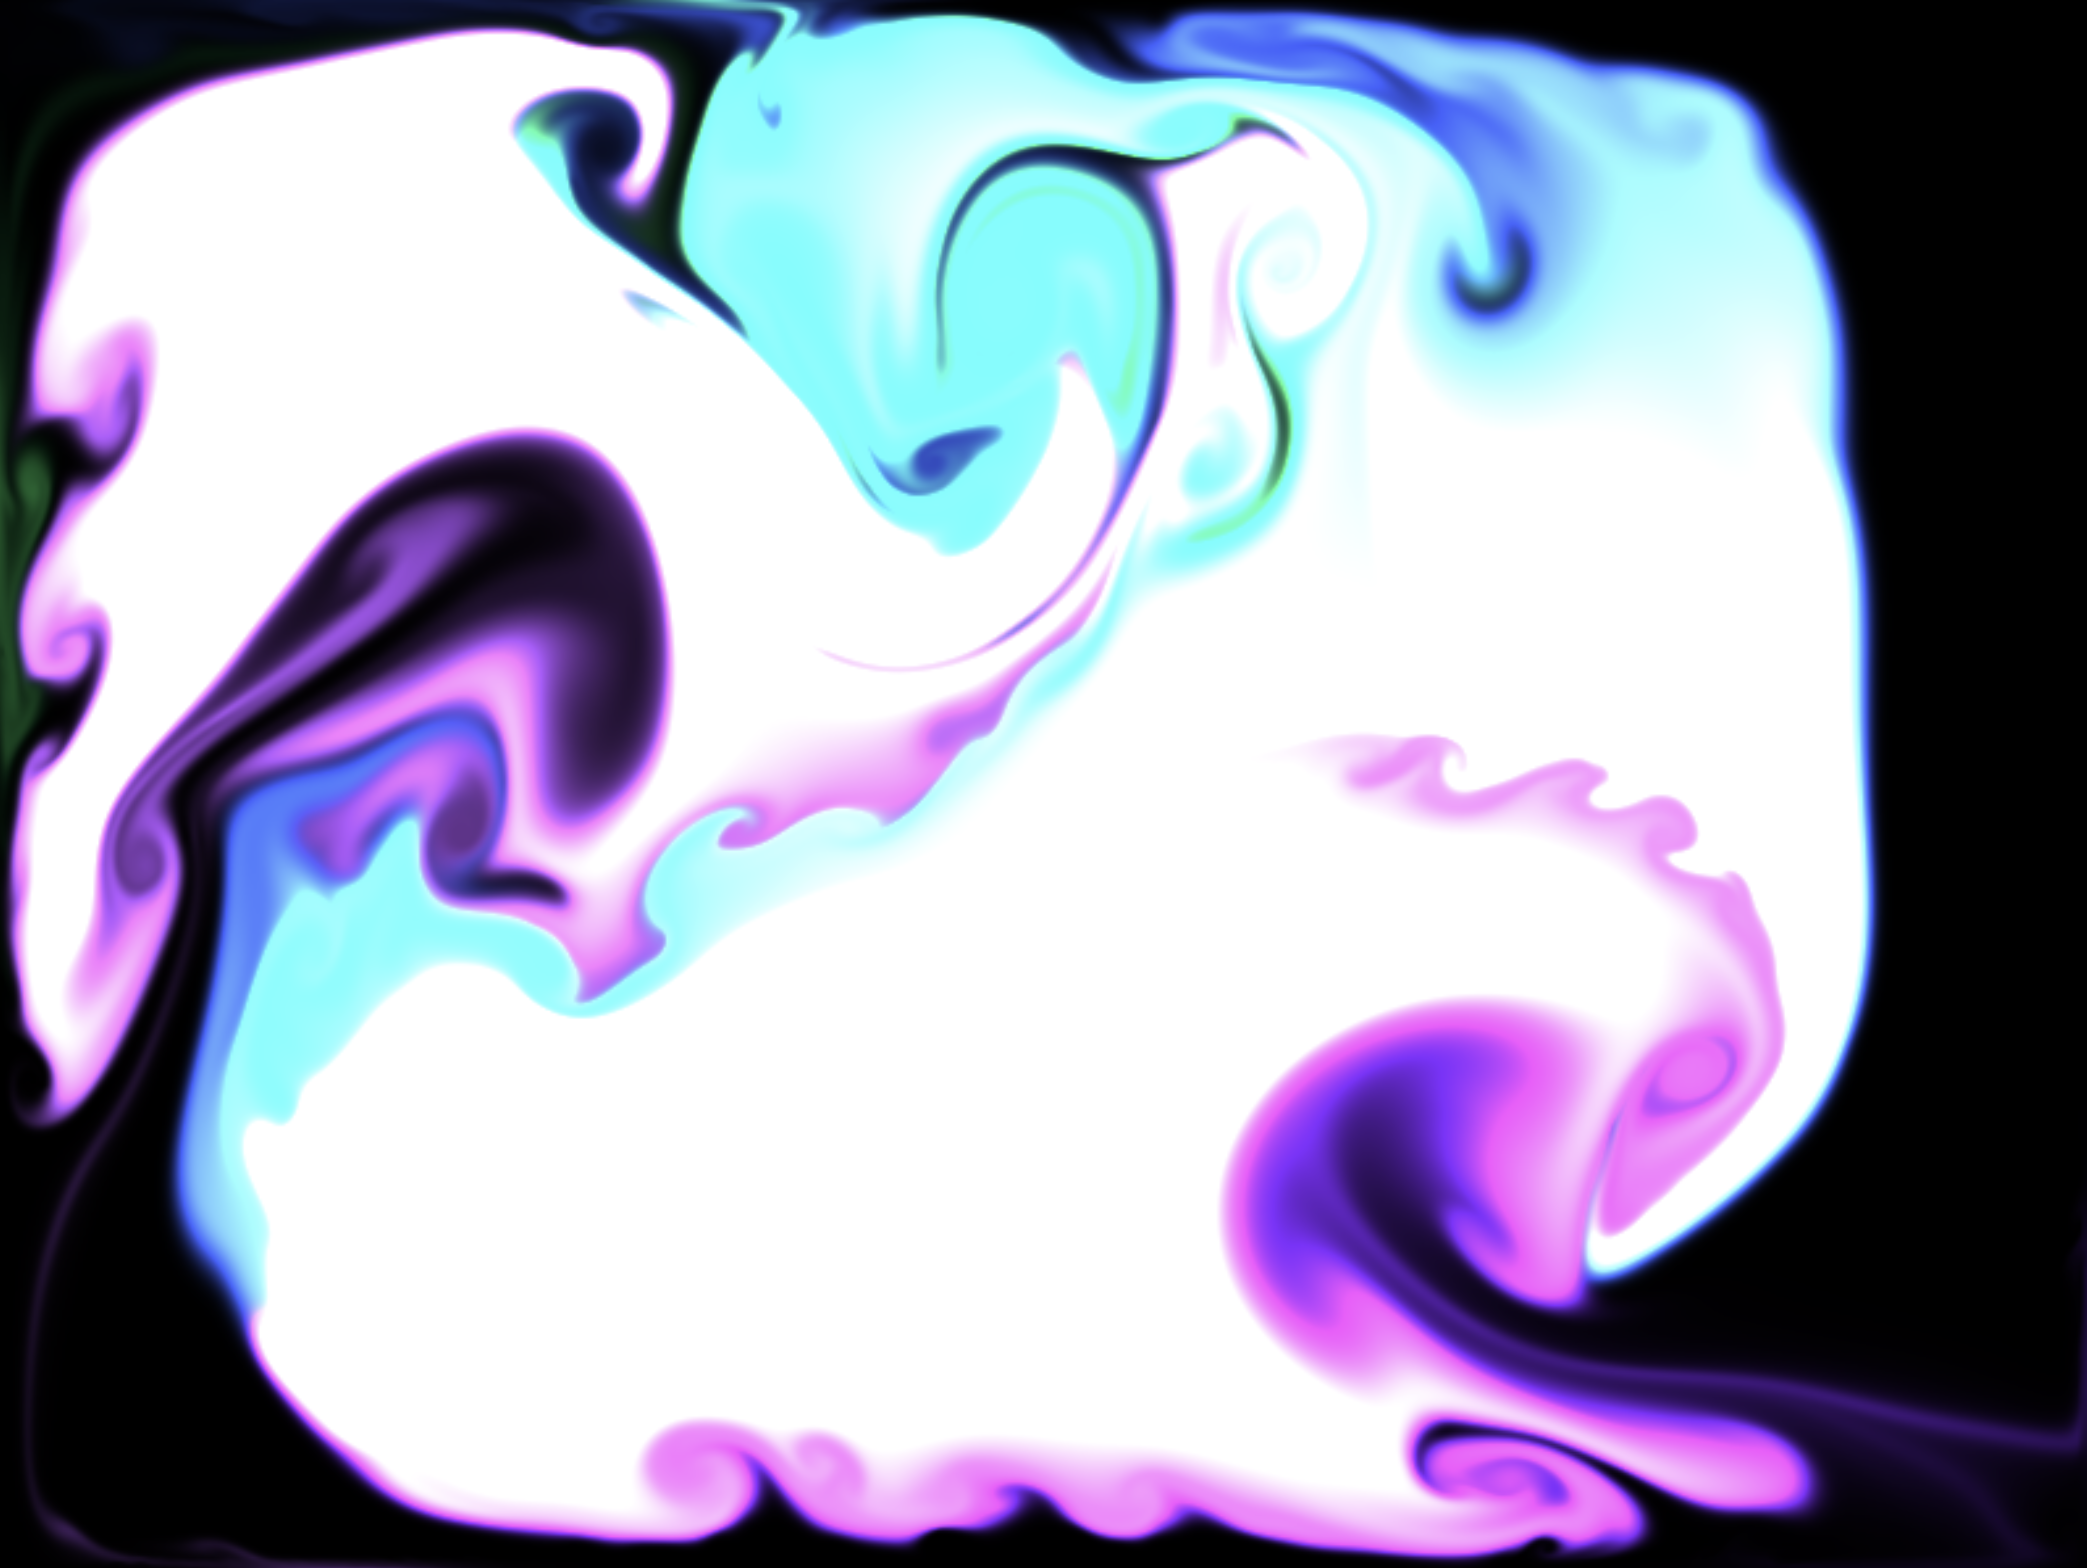
\includegraphics[width=\linewidth]{result.png}
  \caption{A screenshot of the resulting simulation.}
  \label{fig:result}
\end{figure}

There are some issues, that could be fixed with a bit more work.
Firstly, there is an issues where the edges actually seem porous and fluid seems to ``seep'' through them.
This is most likely a result of the back-tracing way that advection is done, and should be resolved.
Due to the same issue, fluids that touch a boundary will seem to ``flow in'' from that direction forever
when there is a force acting away from that boundary.

Secondly, this method could be extended to three-dimensions with relative ease, and was originally planned to be.
It was not, however, due to time constraints.

\section{Summary}

In summary, this project created a (mostly) successful implementation of a two-dimensional continuos fluid
in WebGL.
The Jacobi method for estimating the pressure equation proved fast and accurate enough for 
this 2D visual simulation.

The author was impressed by how easily textures could be used as the fluid ``particles'',
and the usual assembly step skipped. 
Furthermore, the author finds that WebGL is a great framework for physics-based simulation development
due to its relative ease in set-up, deployment and OS-independence.

% Bibliography
\bibliographystyle{ACM-Reference-Format}
\bibliography{paper}



\end{document}
